\section{Problem Overview}
\label{sec:overview}

\subsection{The 2 Sorts of Linked Text}
We begin by breaking down the two sorts of linked text that the developer will
be interested in generating. 

\begin{figure}
   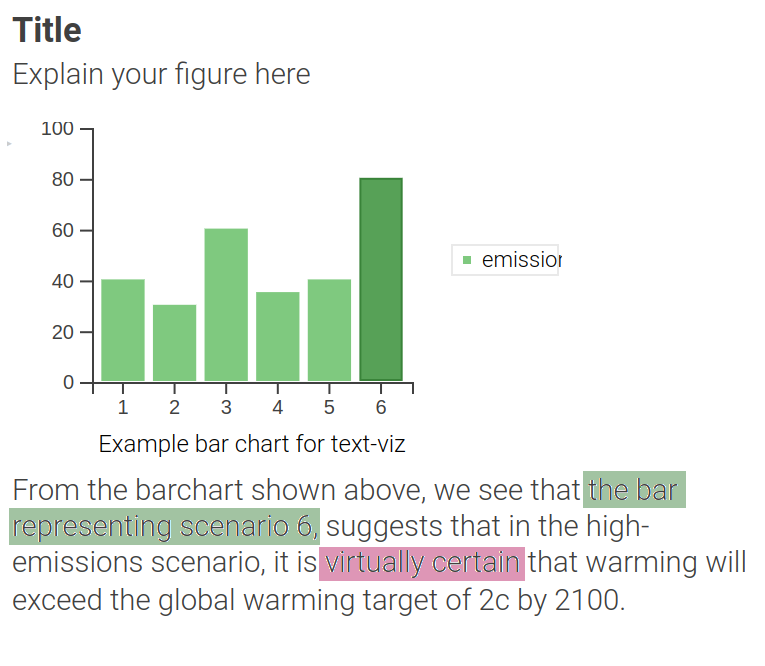
\includegraphics[width=0.7\textwidth]{fig/text-viz-types.png}
   \caption{Two sorts of linked text}
   \label{fig:linked-text-types}
\end{figure}

\subsubsection{Direct Reference To Visual Elements}
The first sort of linked text is a direct reference to a visual element. In 
\figref{linked-text-types}, this corresponds to the text which has been highlighted
in green, referring to the darker bar in the barchart. In situations like this, the
developer is likely to know the exact text they want to be linked ahead of time.
To construct the linking, the system needs to be able to identify the variable that
represents the visual element in question.  It must then synthesize a function which "describes"
the visual element in question, ie returns the string of text the author has identified as 
needing to be linked.

\subsubsection{Indirect Summary of Underlying Data}
The second sort of linked text is summarizing some underlying data. In \figref{linked-text-types},
the text that has been highlighted in pink is an example of this. The text has been synthesized
by comparing a (spoofed) probability against a map of calibrated terminology. By this we mean that
probabilities within certain ranges are given simple natural language descriptions. ``Virtually certain'
is a term used by the IPCC to describe probabilities between 99\% and 100\%. The system should be able
to synthesize such a mapping and insert a call to this mapping into a text field. Once such a mapping
has been synthesized, the system should be able to reuse it where appropriate, so in this example if
we wanted to refer to a different probability, we should not synthesize a new mapping, just insert
a new call to the mapping in the appropriate location. For now, we call these mappings "policies".

\subsection{Kinds of Policy}
Here we shall present some examples of the type of policy that we might want to synthesize.

\paragraph{Calibrated Terminology:} in scientific reporting, probabilities are often not directly given, but instead
mapped to calibrated terminology. We have already mentioned the term ``virtually certain'' from the IPCC report, but in the beginning
of that document, they make sure to explain the meaning of terms like ``likely'' and ``very likely'' as well. This
sort of simple conversion is an example of the simplest form of policy that one might want to synthesize.